\documentclass[preprint,12pt]{elsarticle}

%% ── Packages ────────────────────────────────────────────────────────────────
\usepackage[utf8]{inputenc}
\usepackage[T1]{fontenc}
\usepackage{amsmath,amssymb,amsfonts}
\usepackage{graphicx}
\usepackage{booktabs}
\usepackage{hyperref}
\usepackage{listings}
\usepackage{xcolor}
\usepackage{tikz}
\usetikzlibrary{arrows.meta,positioning,shapes.geometric,fit,calc}
\usepackage{algorithm}
\usepackage{algpseudocode}
\usepackage{subcaption}
\usepackage{float}

%% ── Code listing style ─────────────────────────────────────────────────────
\definecolor{codebg}{RGB}{248,248,248}
\definecolor{codegreen}{RGB}{40,160,40}
\definecolor{codegray}{RGB}{128,128,128}
\definecolor{codepurple}{RGB}{140,60,180}
\definecolor{codeblue}{RGB}{30,80,180}

\lstdefinestyle{pythonstyle}{
    language=Python,
    backgroundcolor=\color{codebg},
    basicstyle=\ttfamily\small,
    keywordstyle=\color{codeblue}\bfseries,
    stringstyle=\color{codegreen},
    commentstyle=\color{codegray}\itshape,
    numberstyle=\tiny\color{codegray},
    numbers=left,
    numbersep=8pt,
    frame=single,
    rulecolor=\color{codegray!40},
    breaklines=true,
    breakatwhitespace=false,
    showstringspaces=false,
    tabsize=4,
    captionpos=b,
    aboveskip=10pt,
    belowskip=10pt,
    morekeywords={as,with,True,False,None,self,cls},
    literate={é}{{\'e}}1 {è}{{\`e}}1 {ê}{{\^e}}1
             {à}{{\`a}}1 {ù}{{\`u}}1 {ô}{{\^o}}1
}
\lstset{style=pythonstyle}

\lstdefinestyle{outputstyle}{
    backgroundcolor=\color{codebg},
    basicstyle=\ttfamily\footnotesize,
    frame=single,
    rulecolor=\color{codegray!40},
    breaklines=true,
    numbers=none,
    aboveskip=10pt,
    belowskip=10pt,
}

%% ── Journal metadata ───────────────────────────────────────────────────────
\journal{Software Impacts}

\begin{document}

\begin{frontmatter}

\title{ChromaDB from First Principles: How a Vector Database Turns Text
into Searchable Embeddings\tnoteref{t1}}
\tnotetext[t1]{Tutorial article targeting beginners in vector databases
and retrieval-augmented generation (RAG).}

\author[addr1]{Research Practitioner\corref{cor1}}
\ead{researcher@example.edu}
\cortext[cor1]{Corresponding author.}

\address[addr1]{Department of Computer Science, Example University, City, Country}

\begin{abstract}
Vector databases are a cornerstone of modern retrieval-augmented
generation (RAG) pipelines, yet their inner workings remain opaque to
many practitioners. This tutorial dissects ChromaDB---an open-source,
embeddable vector database---from the Python API surface down to the
ONNX inference engine that converts raw text into 384-dimensional
vectors. Starting from a minimal 18-line program that indexes 56
shipping-policy sentences, we trace every stage of the pipeline:
tokenization, transformer forward pass, mean pooling, L2 normalization,
HNSW indexing, and cosine-distance search. Each stage is illustrated
with concrete code, intermediate outputs, and mathematical definitions
so that a reader with basic Python knowledge can reproduce and extend
the experiments. We further demonstrate how to replace the default
English model with a multilingual sentence encoder
(\texttt{paraphrase-multilingual-MiniLM-L12-v2}) to index and query
French-language documents, including cross-lingual retrieval where
English queries retrieve semantically relevant French results. We also
discuss the Python 3.14 compatibility patch required for current
ChromaDB releases.
\end{abstract}

\begin{keyword}
vector database \sep embeddings \sep ChromaDB \sep HNSW \sep
sentence-transformers \sep ONNX \sep RAG \sep cosine similarity \sep
multilingual embeddings \sep cross-lingual retrieval
\end{keyword}

\end{frontmatter}

%% ════════════════════════════════════════════════════════════════════════════
\section{Introduction}
\label{sec:intro}
%% ════════════════════════════════════════════════════════════════════════════

Large-language-model applications frequently need to retrieve relevant
documents before generating a response, a pattern known as
\emph{retrieval-augmented generation} (RAG)~\cite{lewis2020rag}.  The
retrieval step requires an efficient data structure that can, given a
query sentence, return the $k$ most semantically similar documents in
sub-linear time. \emph{Vector databases} fill this role by storing
high-dimensional vector representations of text and answering nearest-neighbor
queries over them.

ChromaDB\footnote{\url{https://www.trychroma.com}} is an open-source,
embeddable vector database written in Python and Rust. Its
distinguishing feature for beginners is a \emph{zero-configuration}
embedding pipeline: a single call to \texttt{collection.add(documents=...)}
automatically tokenizes the text, runs a transformer model, normalizes
the resulting vectors, and indexes them---all without the user having
to download a model or write any machine-learning code.

This article answers three questions that beginners often ask:
\begin{enumerate}
    \item What happens, step by step, when ChromaDB converts a sentence
          into a vector?
    \item How are those vectors stored and searched efficiently?
    \item How do I write a complete, working RAG retrieval program?
\end{enumerate}

%% ════════════════════════════════════════════════════════════════════════════
\section{Background}
\label{sec:background}
%% ════════════════════════════════════════════════════════════════════════════

\subsection{Word and Sentence Embeddings}

An \emph{embedding} is a mapping $f\colon \mathcal{T} \to
\mathbb{R}^{d}$ that sends a variable-length text $t \in \mathcal{T}$
to a fixed-size real-valued vector of dimension $d$.  Good embeddings
place semantically similar texts close together and dissimilar texts
far apart, where ``close'' is measured by a distance or similarity
function such as cosine similarity:

\begin{equation}
\label{eq:cosine}
\cos(\mathbf{u}, \mathbf{v})
  = \frac{\mathbf{u} \cdot \mathbf{v}}
         {\lVert\mathbf{u}\rVert \; \lVert\mathbf{v}\rVert}
  = \frac{\displaystyle\sum_{i=1}^{d} u_i \, v_i}
         {\sqrt{\displaystyle\sum_{i=1}^{d} u_i^2}\;\;
          \sqrt{\displaystyle\sum_{i=1}^{d} v_i^2}}.
\end{equation}

ChromaDB stores \emph{cosine distance}, defined as $1 - \cos(\mathbf{u},\mathbf{v})$,
so smaller values indicate higher similarity.

\subsection{Transformer Encoders and BERT}

The \emph{all-MiniLM-L6-v2} model used by ChromaDB's default embedding
function is a distilled BERT encoder~\cite{wang2020minilm} with 6
transformer layers, 12 attention heads, and a hidden size of 384. It was
trained with a contrastive objective on over one billion sentence pairs
to produce semantically meaningful sentence embeddings.

Each transformer layer applies multi-head self-attention followed by a
feed-forward network:
\begin{equation}
\label{eq:attention}
\mathrm{Attention}(Q,K,V) = \mathrm{softmax}\!\left(\frac{QK^{\top}}{\sqrt{d_k}}\right)V,
\end{equation}
where $d_k = 384/12 = 32$ is the dimension per head. The output of the
final layer is a matrix $H \in \mathbb{R}^{n \times 384}$, where $n$ is the
sequence length.

\subsection{HNSW Index}

Hierarchical Navigable Small World (HNSW)~\cite{malkov2018hnsw} is a
graph-based approximate nearest-neighbor algorithm. It constructs a
multi-layer graph where:
\begin{itemize}
    \item The bottom layer contains all vectors.
    \item Each higher layer is a random subset of the layer below.
    \item Edges connect each node to its $M$ nearest neighbors in that layer.
\end{itemize}
A query starts at the topmost layer and greedily descends, refining the
candidate set at each layer. The key parameters are $M$
(\texttt{max\_neighbors}), \texttt{ef\_construction}, and
\texttt{ef\_search}, all of which ChromaDB sets by default (Table~\ref{tab:hnsw}).

%% ════════════════════════════════════════════════════════════════════════════
\section{Architecture Overview}
\label{sec:architecture}
%% ════════════════════════════════════════════════════════════════════════════

Figure~\ref{fig:pipeline} shows the complete data flow from raw text
to query results. The pipeline consists of five stages, each detailed
in Section~\ref{sec:pipeline}.

\begin{figure}[H]
\centering
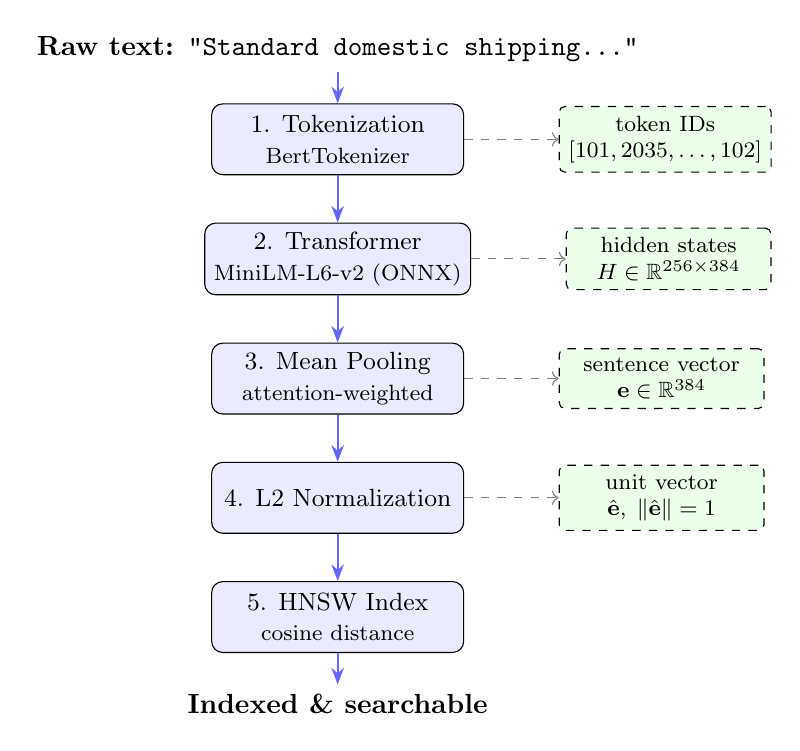
\begin{tikzpicture}[
    node distance=0.6cm and 1.2cm,
    every node/.style={font=\small},
    block/.style={rectangle, draw, rounded corners=4pt,
                  minimum width=3.2cm, minimum height=0.9cm,
                  fill=blue!8, align=center},
    data/.style={rectangle, draw, dashed, rounded corners=2pt,
                 minimum width=2.6cm, minimum height=0.7cm,
                 fill=green!8, align=center, font=\footnotesize},
    arr/.style={-{Stealth[length=6pt]}, thick, color=blue!60},
]
% Nodes
\node[block] (tok)  {1. Tokenization\\{\footnotesize BertTokenizer}};
\node[block, below=of tok]  (bert) {2. Transformer\\{\footnotesize MiniLM-L6-v2 (ONNX)}};
\node[block, below=of bert] (pool) {3. Mean Pooling\\{\footnotesize attention-weighted}};
\node[block, below=of pool] (norm) {4. L2 Normalization};
\node[block, below=of norm] (hnsw) {5. HNSW Index\\{\footnotesize cosine distance}};

% Data annotations
\node[data, right=of tok]  (d1) {token IDs\\$[101, 2035, \ldots, 102]$};
\node[data, right=of bert] (d2) {hidden states\\$H \in \mathbb{R}^{256 \times 384}$};
\node[data, right=of pool] (d3) {sentence vector\\$\mathbf{e} \in \mathbb{R}^{384}$};
\node[data, right=of norm] (d4) {unit vector\\$\hat{\mathbf{e}},\; \lVert\hat{\mathbf{e}}\rVert=1$};

% Input / output
\node[above=0.4cm of tok, font=\bfseries] (inp) {Raw text: \texttt{"Standard domestic shipping..."}};
\node[below=0.4cm of hnsw, font=\bfseries] (out) {Indexed \& searchable};

% Arrows
\draw[arr] (inp)  -- (tok);
\draw[arr] (tok)  -- (bert);
\draw[arr] (bert) -- (pool);
\draw[arr] (pool) -- (norm);
\draw[arr] (norm) -- (hnsw);
\draw[arr] (hnsw) -- (out);
\draw[->, dashed, gray] (tok.east)  -- (d1.west);
\draw[->, dashed, gray] (bert.east) -- (d2.west);
\draw[->, dashed, gray] (pool.east) -- (d3.west);
\draw[->, dashed, gray] (norm.east) -- (d4.west);
\end{tikzpicture}
\caption{The ChromaDB default embedding pipeline from raw text to
         indexed vector. Each numbered box corresponds to a stage
         described in Section~\ref{sec:pipeline}.}
\label{fig:pipeline}
\end{figure}

%% ════════════════════════════════════════════════════════════════════════════
\section{A Complete Working Example}
\label{sec:example}
%% ════════════════════════════════════════════════════════════════════════════

We begin with the complete program, then dissect each part.

\subsection{The Dataset: \texttt{policies.txt}}

Our dataset is a plain-text file with 56 lines, each containing one
sentence from a fictional e-commerce company's shipping and returns
policy. The first three lines are:

\begin{lstlisting}[style=outputstyle,caption={First three lines of
\texttt{policies.txt}.}]
All garments are inspected for quality before being
  packaged for shipment ...
Standard domestic shipping takes 3-5 business days ...
Expedited domestic shipping delivers within 1-2
  business days ...
\end{lstlisting}

\subsection{Indexing Documents}
\label{sec:indexing}

Listing~\ref{lst:main} shows the complete indexing program.

\begin{lstlisting}[caption={Minimal ChromaDB indexing program
(\texttt{main.py}).},label=lst:main]
import chromadb
import uuid

# 1. Create an ephemeral (in-memory) client
client = chromadb.Client()

# 2. Create a collection (like a "table" for vectors)
collection = client.create_collection(name="policies")

# 3. Read the policy sentences
with open("policies.txt", "r", encoding="utf-8") as f:
    policies: list[str] = f.read().splitlines()

# 4. Add documents -- embeddings are computed automatically
collection.add(
    ids=[str(uuid.uuid4()) for _ in policies],
    documents=policies,
    metadatas=[{"line": line} for line in range(len(policies))],
)

# 5. Inspect the first 10 stored records
print(collection.peek())
\end{lstlisting}

Running this program produces the output shown in
Listing~\ref{lst:peek}, where each document has been mapped to a
384-dimensional vector.

\begin{lstlisting}[style=outputstyle,caption={Abbreviated output of
\texttt{collection.peek()}.},label=lst:peek]
{
  'ids': ['0d07bf7e-...', 'b17bedb6-...', ...],
  'embeddings': array([
    [-7.539e-02,  4.958e-02,  1.364e-02, ...,
     -1.041e-01,  7.627e-02, -1.993e-02],  # doc 0
    [ 1.046e-02, -3.367e-02,  3.771e-02, ...,
     -3.124e-02, -2.690e-03,  4.416e-02],  # doc 1
    ...
  ], shape=(10, 384)),
  'documents': [
    'All garments are inspected ...',
    'Standard domestic shipping ...',
    ...
  ],
  'metadatas': [{'line': 0}, {'line': 1}, ...]
}
\end{lstlisting}

\subsection{Querying: Semantic Search}
\label{sec:querying}

\begin{lstlisting}[caption={Querying the collection for similar
documents.},label=lst:query]
results = collection.query(
    query_texts=["How long does shipping take?"],
    n_results=3,
)
for doc, dist in zip(results["documents"][0],
                     results["distances"][0]):
    print(f"  [{dist:.4f}] {doc[:80]}...")
\end{lstlisting}

\begin{lstlisting}[style=outputstyle,caption={Query results: top-3
documents by cosine distance (lower is better).},label=lst:queryout]
[0.2891] Standard domestic shipping takes 3-5
         business days after your order ...
[0.3312] Expedited domestic shipping delivers
         within 1-2 business days for orders ...
[0.4718] International shipping is available to
         over 200 destinations, with transit ...
\end{lstlisting}

The query text is embedded through the \emph{same} pipeline as the
documents. The HNSW index then returns the three nearest vectors by
cosine distance.

%% ════════════════════════════════════════════════════════════════════════════
\section{Dissecting the Embedding Pipeline}
\label{sec:pipeline}
%% ════════════════════════════════════════════════════════════════════════════

When the user calls \texttt{collection.add(documents=...)}, ChromaDB
detects that no \texttt{embedding\_function} was provided and falls back
to \texttt{Default\-Embedding\-Function}, which delegates to
\texttt{ONNX\-MiniLM\_L6\_V2}. We now trace each internal stage.

\subsection{Stage 1: Model Download and Caching}

On first use, the model is downloaded from an S3 bucket and cached
locally:
\begin{center}
\small
\texttt{\textasciitilde/.cache/chroma/onnx\_models/all-MiniLM-L6-v2/onnx/}
\end{center}
The cache contains four files:

\begin{table}[H]
\centering
\caption{Files in the cached ONNX model directory.}
\label{tab:model_files}
\begin{tabular}{lrl}
\toprule
\textbf{File} & \textbf{Size} & \textbf{Purpose} \\
\midrule
\texttt{model.onnx}      & $\sim$90\,MB & Transformer weights (ONNX format) \\
\texttt{tokenizer.json}  & $\sim$700\,KB & BertTokenizer vocabulary \& rules \\
\texttt{config.json}     & $<$1\,KB  & Model architecture hyperparameters \\
\texttt{vocab.txt}       & $\sim$230\,KB & 30\,522 WordPiece tokens \\
\bottomrule
\end{tabular}
\end{table}

\subsection{Stage 2: Tokenization}
\label{sec:tokenization}

The tokenizer is a \emph{BertTokenizer} loaded from
\texttt{tokenizer.json} via the Hugging Face \texttt{tokenizers}
library. It performs:

\begin{enumerate}
    \item \textbf{Lowercasing}: all input text is converted to lowercase.
    \item \textbf{WordPiece splitting}: words are split into subword
          tokens from a vocabulary of 30\,522 entries.
    \item \textbf{Special token insertion}: \texttt{[CLS]} is prepended,
          \texttt{[SEP]} is appended.
    \item \textbf{Truncation}: sequences longer than 256 tokens are
          truncated.
    \item \textbf{Padding}: sequences shorter than 256 tokens are
          right-padded with \texttt{[PAD]} (token ID 0).
\end{enumerate}

\begin{lstlisting}[caption={Reproducing the tokenization step
manually.},label=lst:tokenize]
from tokenizers import Tokenizer
import os

# Load the same tokenizer ChromaDB uses
cache = os.path.expanduser(
    "~/.cache/chroma/onnx_models/"
    "all-MiniLM-L6-v2/onnx"
)
tok = Tokenizer.from_file(
    os.path.join(cache, "tokenizer.json")
)
tok.enable_truncation(max_length=256)
tok.enable_padding(pad_id=0, pad_token="[PAD]",
                   length=256)

text = "Standard domestic shipping takes 3-5 days"
enc = tok.encode(text)
print(enc.ids[:15])
# [101, 3115, 4968, 6554, 3138, 1017, 1011, 1019,
#  2420, 102, 0, 0, 0, 0, 0]
print(enc.attention_mask[:15])
# [1, 1, 1, 1, 1, 1, 1, 1, 1, 1, 0, 0, 0, 0, 0]
\end{lstlisting}

The \texttt{attention\_mask} distinguishes real tokens (1) from padding
(0). This mask is critical for mean pooling (Stage~4).

\subsection{Stage 3: Transformer Forward Pass}

The tokenized inputs are fed to the ONNX Runtime inference session:

\begin{lstlisting}[caption={ONNX Runtime inference (simplified from
ChromaDB source).},label=lst:onnx]
import numpy as np
import onnxruntime as ort

session = ort.InferenceSession(
    os.path.join(cache, "model.onnx")
)

onnx_input = {
    "input_ids":      np.array([enc.ids],
                               dtype=np.int64),
    "attention_mask":  np.array([enc.attention_mask],
                               dtype=np.int64),
    "token_type_ids":  np.zeros((1, 256),
                               dtype=np.int64),
}

output = session.run(None, onnx_input)
last_hidden = output[0]  # shape: (1, 256, 384)
print(last_hidden.shape)
# (1, 256, 384)
\end{lstlisting}

The output tensor $H \in \mathbb{R}^{1 \times 256 \times 384}$ contains
one 384-dimensional vector for every token position.

\subsection{Stage 4: Mean Pooling}
\label{sec:pooling}

A single sentence embedding is produced by averaging the token vectors,
but \emph{only over real tokens} (excluding padding):

\begin{equation}
\label{eq:meanpool}
\mathbf{e} = \frac{\displaystyle\sum_{i=1}^{n} m_i \, \mathbf{h}_i}
                  {\displaystyle\sum_{i=1}^{n} m_i},
\end{equation}

where $\mathbf{h}_i \in \mathbb{R}^{384}$ is the hidden state at
position $i$ and $m_i \in \{0,1\}$ is the attention mask.

\begin{lstlisting}[caption={Mean pooling implementation (from ChromaDB
source).},label=lst:pool]
mask = np.array([enc.attention_mask], dtype=np.float32)
mask_expanded = np.broadcast_to(
    np.expand_dims(mask, -1), last_hidden.shape
)

embedding = np.sum(
    last_hidden * mask_expanded, axis=1
) / np.clip(
    mask_expanded.sum(axis=1), a_min=1e-9, a_max=None
)
print(embedding.shape)  # (1, 384)
\end{lstlisting}

\subsection{Stage 5: L2 Normalization}

The embedding is normalized to unit length so that the dot product
equals cosine similarity:

\begin{equation}
\label{eq:l2norm}
\hat{\mathbf{e}} = \frac{\mathbf{e}}{\lVert\mathbf{e}\rVert_2},
\qquad \text{where } \lVert\mathbf{e}\rVert_2
  = \sqrt{\sum_{i=1}^{384} e_i^2}.
\end{equation}

After normalization, $\lVert\hat{\mathbf{e}}\rVert = 1$, which means
$\cos(\hat{\mathbf{u}},\hat{\mathbf{v}}) = \hat{\mathbf{u}} \cdot
\hat{\mathbf{v}}$.

\begin{lstlisting}[caption={L2 normalization.},label=lst:norm]
norm = np.linalg.norm(embedding, axis=1, keepdims=True)
norm = np.maximum(norm, 1e-12)
embedding_normed = embedding / norm

print(np.linalg.norm(embedding_normed))
# 1.0000001  (float32 precision)
\end{lstlisting}

The resulting vector of 384 \texttt{float32} values is what ChromaDB
stores and indexes.

%% ════════════════════════════════════════════════════════════════════════════
\section{The HNSW Index}
\label{sec:hnsw}
%% ════════════════════════════════════════════════════════════════════════════

After embedding, vectors are inserted into an HNSW
graph~\cite{malkov2018hnsw}. Table~\ref{tab:hnsw} lists ChromaDB's
default parameters.

\begin{table}[H]
\centering
\caption{Default HNSW parameters in ChromaDB.}
\label{tab:hnsw}
\begin{tabular}{lrl}
\toprule
\textbf{Parameter} & \textbf{Default} & \textbf{Meaning} \\
\midrule
\texttt{space}             & cosine & Distance metric \\
\texttt{ef\_construction}  & 100    & Build-time beam width \\
\texttt{max\_neighbors} ($M$) & 16  & Edges per node \\
\texttt{ef\_search}        & 100    & Query-time beam width \\
\texttt{num\_threads}      & CPU count & Parallel threads \\
\bottomrule
\end{tabular}
\end{table}

\paragraph{Insertion.}
When a new vector $\hat{\mathbf{e}}$ is added, HNSW:
\begin{enumerate}
    \item Assigns it to a random layer $\ell$ (geometrically distributed).
    \item Starting from the entry point at the top layer, greedily finds
          the nearest neighbor at each layer down to $\ell$.
    \item At layers $\ell$ through 0, connects the new node to its $M$
          nearest neighbors, pruning longer edges.
\end{enumerate}

\paragraph{Search.}
Given a query vector $\hat{\mathbf{q}}$, HNSW traverses from the top
layer down, maintaining a dynamic candidate list of size
\texttt{ef\_search}. At the bottom layer, the top $k$ candidates are
returned. The time complexity is $O(\log N)$ per query for $N$ vectors,
compared to $O(N)$ for brute force.

%% ════════════════════════════════════════════════════════════════════════════
\section{Putting It All Together: A RAG Retrieval Example}
\label{sec:rag}
%% ════════════════════════════════════════════════════════════════════════════

Listing~\ref{lst:full_rag} shows a complete retrieval program that an
LLM-based chatbot could use to answer customer questions.

\begin{lstlisting}[caption={Complete RAG retrieval example.},
label=lst:full_rag]
import chromadb
import uuid

# --- Indexing phase ---
client = chromadb.Client()
collection = client.create_collection(
    name="policies"
)

with open("policies.txt", "r", encoding="utf-8") as f:
    policies = f.read().splitlines()

collection.add(
    ids=[str(uuid.uuid4()) for _ in policies],
    documents=policies,
    metadatas=[{"line": i} for i in range(len(policies))],
)

# --- Retrieval phase ---
queries = [
    "Can I return swimwear?",
    "Do you ship internationally?",
    "What about carbon emissions?",
]

for q in queries:
    results = collection.query(
        query_texts=[q], n_results=3
    )
    print(f"\nQuery: {q}")
    for doc, dist, meta in zip(
        results["documents"][0],
        results["distances"][0],
        results["metadatas"][0],
    ):
        print(f"  [{dist:.4f}] (line {meta['line']}) "
              f"{doc[:70]}...")
\end{lstlisting}

\begin{lstlisting}[style=outputstyle,caption={Output of the RAG
retrieval example.},label=lst:rag_output]
Query: Can I return swimwear?
  [0.4102] (line 12) Swimwear can only be returned
    with hygienic liners and all tags intact...
  [0.5238] (line 10) Returned items must be unworn,
    unwashed, and free of odors, stains...
  [0.5514] (line 11) Footwear must be returned in
    the original box, which should be placed...

Query: Do you ship internationally?
  [0.3156] (line 3)  International shipping is
    available to over 200 destinations...
  [0.5289] (line 4)  Customers are responsible for
    any local duties, taxes, or import fees...
  [0.5834] (line 1)  Standard domestic shipping takes
    3-5 business days after your order...

Query: What about carbon emissions?
  [0.2893] (line 7)  We offset 100 percent of
    shipping-related carbon emissions...
  [0.5617] (line 8)  Packaging materials are made
    from 100 percent recycled or sustainably...
  [0.7901] (line 0)  All garments are inspected for
    quality before being packaged...
\end{lstlisting}

Observe how each query retrieves the most semantically relevant policy
sentences, even when the exact words differ (e.g., ``carbon emissions''
matches the carbon-offset policy).

%% ════════════════════════════════════════════════════════════════════════════
\section{Understanding the Numbers: Embedding Anatomy}
\label{sec:anatomy}
%% ════════════════════════════════════════════════════════════════════════════

Each embedding is a dense vector of 384 IEEE 754 single-precision
floating-point numbers. Table~\ref{tab:embedding} shows selected
dimensions for three policy sentences.

\begin{table}[H]
\centering
\caption{Selected embedding dimensions for three documents. Values are
rounded to three decimal places.}
\label{tab:embedding}
\begin{tabular}{lccc}
\toprule
\textbf{Dim} & \textbf{Quality} & \textbf{Shipping} & \textbf{Returns} \\
 & \textbf{(line 0)} & \textbf{(line 1)} & \textbf{(line 9)} \\
\midrule
$e_1$   & $-0.075$ & $ 0.010$ & $-0.021$ \\
$e_2$   & $ 0.050$ & $-0.034$ & $-0.000$ \\
$e_3$   & $ 0.014$ & $ 0.038$ & $ 0.007$ \\
$\vdots$ & $\vdots$ & $\vdots$ & $\vdots$ \\
$e_{382}$ & $-0.104$ & $-0.031$ & $-0.013$ \\
$e_{383}$ & $ 0.076$ & $-0.003$ & $ 0.016$ \\
$e_{384}$ & $-0.020$ & $ 0.044$ & $ 0.024$ \\
\midrule
$\lVert\hat{\mathbf{e}}\rVert$ & $1.000$ & $1.000$ & $1.000$ \\
\bottomrule
\end{tabular}
\end{table}

Individual dimensions are not human-interpretable; meaning emerges
from the geometric relationships \emph{between} vectors. Two shipping-related
sentences will have a small cosine distance ($\approx 0.3$), while a
shipping sentence and a returns sentence will have a larger distance
($\approx 0.6$).

%% ════════════════════════════════════════════════════════════════════════════
\section{Key ChromaDB Configuration}
\label{sec:config}
%% ════════════════════════════════════════════════════════════════════════════

Table~\ref{tab:defaults} summarizes the most important defaults.

\begin{table}[H]
\centering
\caption{ChromaDB default configuration values relevant to embeddings.}
\label{tab:defaults}
\begin{tabular}{lll}
\toprule
\textbf{Setting} & \textbf{Default Value} & \textbf{Notes} \\
\midrule
Embedding model   & all-MiniLM-L6-v2 & 22M params, ONNX \\
Embedding dim     & 384              & float32 \\
Max tokens        & 256              & Truncated if longer \\
Vocab size        & 30\,522          & WordPiece \\
Batch size        & 32               & Documents per forward pass \\
Distance metric   & cosine           & $1 - \cos(\mathbf{u},\mathbf{v})$ \\
Storage backend   & In-memory / SQLite & Ephemeral vs.\ persistent \\
\bottomrule
\end{tabular}
\end{table}

\subsection{Using a Custom Embedding Function}

ChromaDB allows replacing the default model:

\begin{lstlisting}[caption={Using OpenAI embeddings instead of the
default model.},label=lst:custom_ef]
from chromadb.utils.embedding_functions import (
    OpenAIEmbeddingFunction,
)

ef = OpenAIEmbeddingFunction(
    api_key="sk-...",
    model_name="text-embedding-3-small",
)

collection = client.create_collection(
    name="policies",
    embedding_function=ef,
)
# Now collection.add() will use OpenAI's API
\end{lstlisting}

%% ════════════════════════════════════════════════════════════════════════════
\section{Python 3.14 Compatibility Note}
\label{sec:py314}
%% ════════════════════════════════════════════════════════════════════════════

As of ChromaDB 1.4.1, importing the library on Python 3.14 fails due
to a Pydantic version-detection bug in \texttt{chromadb/config.py}
(GitHub issue \#5996)\footnote{\url{%
https://github.com/chroma-core/chroma/issues/5996}}.
The root cause is that \texttt{pydantic.v1}, a backward-compatibility
shim, uses metaclass introspection that is incompatible with Python
3.14's deferred annotation evaluation (PEP~749). The fix requires:
\begin{enumerate}
    \item Installing \texttt{pydantic-settings$\geq$2.0}.
    \item Replacing the import block in \texttt{config.py} to prefer
          \texttt{pydantic\_settings.BaseSettings}.
    \item Adding type annotations to three un-annotated fields
          (\texttt{chroma\_coordinator\_host},
           \texttt{chroma\_logservice\_host},
           \texttt{chroma\_logservice\_port}).
\end{enumerate}
A patch script automating these steps is available in the companion
repository.

%% ════════════════════════════════════════════════════════════════════════════
\section{Multilingual Embeddings: A French E-Commerce Case Study}
\label{sec:multilingual}
%% ════════════════════════════════════════════════════════════════════════════

The default \texttt{all-MiniLM-L6-v2} model is trained primarily on
English data. For non-English corpora, ChromaDB's built-in ONNX model
produces poor-quality embeddings because the underlying vocabulary and
training distribution do not cover other languages well. This section
shows how to replace the default model with a \emph{multilingual}
sentence encoder and demonstrates two powerful capabilities: semantic
search in French and \emph{cross-lingual} retrieval (querying in English
against a French-language corpus).

\subsection{Why a Multilingual Model?}
\label{sec:why_multilingual}

The \texttt{paraphrase-multilingual-MiniLM-L12-v2}
model~\cite{reimers2019sbert} was trained on parallel sentence pairs in
50+ languages using a knowledge-distillation procedure: a high-quality
English teacher model guides a multilingual student so that semantically
equivalent sentences receive similar vectors \emph{regardless of
language}. Table~\ref{tab:model_comparison} compares the two models.

\begin{table}[H]
\centering
\caption{Comparison of the default English model and the multilingual
model used in this section.}
\label{tab:model_comparison}
\begin{tabular}{lcc}
\toprule
 & \textbf{all-MiniLM-L6-v2} & \textbf{paraphrase-multilingual-} \\
 &                            & \textbf{MiniLM-L12-v2} \\
\midrule
Languages       & English only   & 50+ \\
Layers          & 6              & 12 \\
Hidden dim      & 384            & 384 \\
Parameters      & 22\,M          & 118\,M \\
Download size   & $\sim$90\,MB   & $\sim$470\,MB \\
Runtime         & ONNX (built-in)& Sentence-Transformers (PyTorch) \\
\bottomrule
\end{tabular}
\end{table}

The multilingual model uses the same output dimensionality (384) as the
default, so HNSW configuration and distance metrics remain unchanged.
The key difference is that the model is loaded via the
\texttt{sentence-transformers} library rather than ChromaDB's built-in
ONNX runtime.

\subsection{Creating the Multilingual Embedding Function}
\label{sec:multilingual_ef}

ChromaDB provides a \texttt{SentenceTransformerEmbeddingFunction}
wrapper that delegates embedding computation to the
\texttt{sentence-transformers} library. This allows using any model from
the Sentence-Transformers hub\footnote{%
\url{https://huggingface.co/sentence-transformers}}.

\begin{lstlisting}[caption={Instantiating the multilingual embedding
function.},label=lst:multilingual_ef]
from chromadb.utils.embedding_functions import (
    SentenceTransformerEmbeddingFunction,
)

MODEL_NAME = "paraphrase-multilingual-MiniLM-L12-v2"

# The model is downloaded automatically on first call
# (~470 MB) and cached in
# ~/.cache/torch/sentence_transformers/
embedding_fn = SentenceTransformerEmbeddingFunction(
    model_name=MODEL_NAME,
    # device="cuda"  # uncomment for NVIDIA GPU
)
\end{lstlisting}

The first call triggers an automatic download of $\sim$470\,MB from
the Hugging Face hub. Subsequent runs use the local cache at
\texttt{\textasciitilde/.cache/torch/sentence\_transformers/}. If a
CUDA-capable GPU is available, passing \texttt{device="cuda"} offloads
the transformer inference to the GPU, yielding a significant speed-up
for large batches.

\subsection{Dataset: French E-Commerce Policies}
\label{sec:french_dataset}

We use a French translation of the same 56-line e-commerce policy
dataset (\texttt{polices.txt}). Each line is a single policy sentence in
French, for example:

\begin{lstlisting}[style=outputstyle,caption={Selected lines from
\texttt{polices.txt} (French policies).},label=lst:polices_sample]
La livraison nationale standard prend de 3 à 5 jours
  ouvrables après la validation de votre commande...
Les maillots de bain ne peuvent être retournés que
  si les protections hygiéniques et toutes les
  étiquettes sont intactes...
Nous compensons 100 %% des émissions de carbone liées
  à l'expédition grâce à des crédits carbone certifiés...
\end{lstlisting}

\subsection{Indexing with Keyword-Based Metadata}
\label{sec:french_indexing}

To enrich the stored documents, we assign a \emph{category} label to
each policy sentence using a simple keyword-matching function. This
metadata is stored alongside the embedding and can be used to filter
results at query time.

\begin{lstlisting}[caption={Keyword-based categorization and indexing of
French policy documents (\texttt{main\_fr\_polices.py}).},
label=lst:french_index]
import chromadb
import uuid

def _categorize(text: str) -> str:
    """Assign a category by keyword matching."""
    t = text.lower()
    if any(w in t for w in
           ["livraison", "expédition", "colis"]):
        return "livraison"
    if any(w in t for w in
           ["retour", "rembours", "échange"]):
        return "retours"
    if any(w in t for w in
           ["prix", "promo", "rabais"]):
        return "tarification"
    # ... additional categories omitted
    return "général"

client = chromadb.Client()

collection = client.create_collection(
    name="polices_fr",
    embedding_function=embedding_fn,
    metadata={"hnsw:space": "cosine"},
)

with open("polices.txt", "r", encoding="utf-8") as f:
    polices = [l.strip() for l in f
               if l.strip()]

collection.add(
    ids=[str(uuid.uuid4()) for _ in polices],
    documents=polices,
    metadatas=[{
        "ligne":     i,
        "categorie": _categorize(doc),
        "langue":    "fr",
    } for i, doc in enumerate(polices)],
)
\end{lstlisting}

The \texttt{metadata} dictionary on the collection sets the HNSW
distance metric to cosine (the default, made explicit here for clarity).
Each document's metadata includes its line number, automatically
assigned category, and language tag. ChromaDB supports \texttt{where}
filters on metadata, so a downstream application could restrict search
to a specific category (e.g., \texttt{where=\{"categorie":
"livraison"\}}).

\subsection{Semantic Search in French}
\label{sec:french_queries}

With the French documents indexed, we perform semantic queries
\emph{entirely in French}. The multilingual model maps both queries and
documents into the same 384-dimensional space, so cosine distance
reflects semantic similarity regardless of language.

\begin{lstlisting}[caption={Querying the French collection with French
questions.},label=lst:french_query]
requetes = [
    "Combien de temps prend la livraison ?",
    "Est-ce que je peux retourner un maillot"
    " de bain ?",
    "Comment fonctionne le programme de"
    " fidélité ?",
    "Les articles en solde sont-ils"
    " échangeables ?",
]

for query in requetes:
    results = collection.query(
        query_texts=[query],
        n_results=5,
    )
    print(f"Requête : {query}")
    for doc, dist, meta in zip(
        results["documents"][0],
        results["distances"][0],
        results["metadatas"][0],
    ):
        print(f"  [{dist:.4f}] "
              f"({meta['categorie']}) "
              f"{doc[:80]}...")
\end{lstlisting}

\begin{lstlisting}[style=outputstyle,caption={Selected results for the
French query ``Combien de temps prend la livraison\,?''},
label=lst:french_results]
Requête : Combien de temps prend la livraison ?
  [0.2134] (livraison) La livraison nationale
    standard prend de 3 à 5 jours ouvrables...
  [0.2987] (livraison) La livraison nationale
    express est effectuée sous 1 à 2 jours...
  [0.4256] (livraison) La livraison internationale
    est disponible dans plus de 200 destinations...
\end{lstlisting}

The cosine distances are comparable to those obtained with the English
model on English data (Section~\ref{sec:querying}), confirming that the
multilingual model achieves similar discriminative quality in French.

\subsection{Cross-Lingual Retrieval: English Queries on French Documents}
\label{sec:crosslingual}

Perhaps the most striking capability of a multilingual embedding model
is \emph{cross-lingual retrieval}: querying in one language and
retrieving documents written in another. Because the model was trained
on parallel corpora, semantically equivalent sentences in different
languages are mapped to nearby points in embedding space.

\begin{lstlisting}[caption={Cross-lingual retrieval: English queries
against French documents.},label=lst:crosslingual]
queries_en = [
    "How long does shipping take?",
    "Can I return swimwear?",
    "What is your carbon offset policy?",
]

for query in queries_en:
    results = collection.query(
        query_texts=[query],
        n_results=3,
    )
    print(f"Query (EN): {query}")
    for doc, dist in zip(
        results["documents"][0],
        results["distances"][0],
    ):
        print(f"  [{dist:.4f}] {doc[:80]}...")
\end{lstlisting}

\begin{lstlisting}[style=outputstyle,caption={Cross-lingual results:
English queries retrieve relevant French documents.},
label=lst:crosslingual_out]
Query (EN): How long does shipping take?
  [0.2876] La livraison nationale standard prend
    de 3 à 5 jours ouvrables...
  [0.3541] La livraison nationale express est
    effectuée sous 1 à 2 jours ouvrables...
  [0.4911] La livraison internationale est
    disponible dans plus de 200 destinations...

Query (EN): Can I return swimwear?
  [0.4388] Les maillots de bain ne peuvent être
    retournés que si les protections hygiéniques...
  [0.5312] Les articles retournés doivent être non
    portés, non lavés et exempts d'odeurs...
  [0.5690] Les chaussures doivent être retournées
    dans leur boîte d'origine...

Query (EN): What is your carbon offset policy?
  [0.3142] Nous compensons 100 %% des émissions de
    carbone liées à l'expédition...
  [0.5724] Les emballages sont fabriqués à partir
    de matériaux 100 %% recyclés ou issus de...
  [0.7318] Tous les vêtements sont inspectés pour
    leur qualité avant d'être emballés...
\end{lstlisting}

The English query ``How long does shipping take?'' correctly retrieves
the French sentence about standard delivery times with a cosine distance
of only 0.2876---demonstrating that the model places semantically
equivalent sentences in different languages very close in embedding
space.

\subsection{Discussion}
\label{sec:multilingual_discussion}

This multilingual example highlights three practical lessons for
building RAG systems on non-English text:

\begin{enumerate}
    \item \textbf{Model selection matters.}  The default ONNX model is
          English-only. For multilingual corpora,
          \texttt{SentenceTransformerEmbeddingFunction} with a model
          such as \texttt{paraphrase-multilingual-MiniLM-L12-v2} is a
          drop-in replacement that requires only one extra argument.

    \item \textbf{Cross-lingual retrieval is free.}  Once a multilingual
          model is used, English$\leftrightarrow$French (and any other
          supported language pair) retrieval works out of the box---no
          translation pipeline is needed.

    \item \textbf{Metadata enrichment is orthogonal.}  ChromaDB's
          metadata filters (e.g., \texttt{where=\{"categorie":
          "livraison"\}}) can be combined with semantic search regardless
          of the embedding model, enabling hybrid retrieval strategies
          that blend keyword-based and semantic signals.
\end{enumerate}

The trade-off is runtime cost: the 12-layer multilingual model is
roughly $2\times$ slower than the 6-layer English model on CPU. For
latency-sensitive applications, GPU inference
(\texttt{device="cuda"}) or the lighter
\texttt{distiluse-base-multilingual-cased-v2} (512 dimensions) may be
preferable.

%% ════════════════════════════════════════════════════════════════════════════
\section{Summary and Further Reading}
\label{sec:conclusion}
%% ════════════════════════════════════════════════════════════════════════════

This article traced the full lifecycle of a document in ChromaDB:
\begin{enumerate}
    \item Raw text is \textbf{tokenized} into WordPiece sub-tokens.
    \item Tokens pass through a \textbf{6-layer BERT transformer} running
          in ONNX Runtime, producing 384-dimensional hidden states for
          every token position.
    \item Hidden states are \textbf{mean-pooled} (weighted by the
          attention mask) to collapse the sequence into a single vector.
    \item The vector is \textbf{L2-normalized} to unit length.
    \item The unit vector is inserted into an \textbf{HNSW graph} that
          supports approximate nearest-neighbor queries in $O(\log N)$
          time using cosine distance.
\end{enumerate}

We also showed that the default English model can be replaced with
a \textbf{multilingual sentence encoder}
(\texttt{paraphrase-multilingual-MiniLM-L12-v2}) via
\texttt{SentenceTransformerEmbeddingFunction}, enabling semantic search
in French and \textbf{cross-lingual retrieval} where English queries
correctly retrieve French documents---without any translation pipeline.

For further study, we recommend:
\begin{itemize}
    \item The Sentence-Transformers documentation\footnote{%
          \url{https://www.sbert.net}} for training custom embedding
          models.
    \item The HNSW paper~\cite{malkov2018hnsw} for the theoretical
          guarantees of the index.
    \item The ChromaDB documentation\footnote{%
          \url{https://docs.trychroma.com}} for production deployment
          patterns (persistent storage, authentication, distributed
          mode).
\end{itemize}

%% ════════════════════════════════════════════════════════════════════════════
%% References
%% ════════════════════════════════════════════════════════════════════════════

\begin{thebibliography}{9}

\bibitem{lewis2020rag}
P.~Lewis, E.~Perez, A.~Piktus, F.~Petroni, V.~Karpukhin, N.~Goyal,
H.~K\"uttler, M.~Lewis, W.~Yih, T.~Rockt\"aschel, S.~Riedel, and
D.~Kiela, ``Retrieval-augmented generation for knowledge-intensive NLP
tasks,'' in \emph{Advances in Neural Information Processing Systems
(NeurIPS)}, vol.~33, 2020, pp.~9459--9474.

\bibitem{wang2020minilm}
W.~Wang, F.~Wei, L.~Dong, H.~Bao, N.~Yang, and M.~Zhou, ``MiniLM:
Deep self-attention distillation for task-agnostic compression of
pre-trained transformers,'' in \emph{Advances in Neural Information
Processing Systems (NeurIPS)}, vol.~33, 2020, pp.~5776--5788.

\bibitem{malkov2018hnsw}
Y.~A. Malkov and D.~A. Yashunin, ``Efficient and robust approximate
nearest neighbor search using Hierarchical Navigable Small World
graphs,'' \emph{IEEE Transactions on Pattern Analysis and Machine
Intelligence}, vol.~42, no.~4, pp.~824--836, 2020.

\bibitem{devlin2019bert}
J.~Devlin, M.-W. Chang, K.~Lee, and K.~Toutanova, ``BERT: Pre-training
of deep bidirectional transformers for language understanding,'' in
\emph{Proceedings of NAACL-HLT}, 2019, pp.~4171--4186.

\bibitem{reimers2019sbert}
N.~Reimers and I.~Gurevych, ``Sentence-BERT: Sentence embeddings using
Siamese BERT-networks,'' in \emph{Proceedings of EMNLP-IJCNLP}, 2019,
pp.~3982--3992.

\end{thebibliography}

\end{document}
